\documentclass[tikz, border=10pt]{standalone}

\usepackage{tikz}
\usetikzlibrary{intersections}

\begin{document}
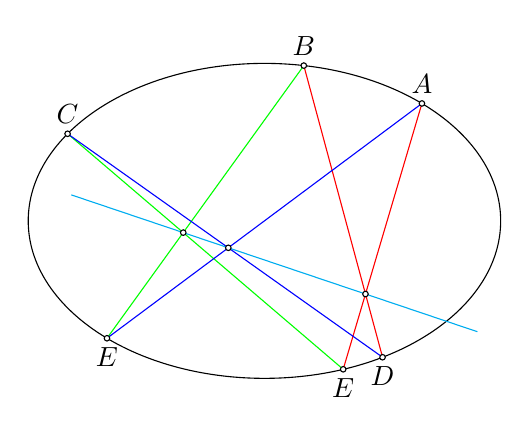
\begin{tikzpicture}
    % draw ellipse
    \draw (0, 0) ellipse (3cm and 2cm);
    % coordinate points
    \coordinate[label=above:$A$] (A) at (2, 1.491);
    \coordinate[label=above:$B$] (B) at (0.5, 1.972);
    \coordinate[label=above:$C$] (C) at (-2.5, 1.106);
    \coordinate[label=below:$D$] (D) at (1.5, -1.732);
    \coordinate[label=below:$E$] (E) at (1, -1.885);
    \coordinate[label=below:$E$] (F) at (-2, -1.491);
    % draw lines
    \draw[red, name path=L1] (A) -- (E);
    \draw[red, name path=L2] (B) -- (D);
    \draw[green, name path=L3] (C) -- (E);
    \draw[green, name path=L4] (B) -- (F);
    \draw[blue, name path=L5] (C) -- (D);
    \draw[blue, name path=L6] (A) -- (F);
    % place intersections
    % L1 and L2
    \begin{scope}[name intersections={of=L1 and L2, name=g}]
        \coordinate[label=30:$ $] (G) at (g-1);
    \end{scope}
    % L3 and L4
    \begin{scope}[name intersections={of=L3 and L4, name=h}]
        \coordinate[label=90:$ $] (H) at (h-1);
    \end{scope}
    % L5 and L6
    \begin{scope}[name intersections={of=L5 and L6, name=k}]
        \coordinate[label=90:$ $] (K) at (k-1);
    \end{scope}
    % pascal's straight line
    \draw[cyan, shorten >=-1.5cm, shorten <=-1.5cm] (G) -- (H);
    % draw small circle points
    \foreach \p in {A, B, C, D, E, F, G, H, K}
        \path[draw, fill=white] (\p) circle (1pt);
\end{tikzpicture}
\end{document}